Following the deformable template paradigm \citep{yuille1991deformable,Grenander1991}, we consider that object instances are obtained by deforming a prototypical object, or `template', through  dense deformation fields. 
This makes it possible  to factor  object variability within a category into variations that are associated to  deformations, generally linked to the object's 2D/3D shape, and variations that are associated to appearance (or, `texture' in graphics), e.g. due to facial hair, skin color, or illumination. 

This factorization largely simplifies the  modelling task. SDMs use it as a stepping stone for the construction of parametric models of deformation and appearance. For instance, in AAMs a combination of Procrustes Analysis, Thin-Plate Spline warping and PCA is the standard pipeline for learning a low-dimensional linear subspace that captures category-specific shape variability \citep{cootes2001active}. Even though we have a common starting point, rather than trying to construct a linear generative model of deformations, we treat the image-to-template correspondence as a vector field that our network tries to regress.

In particular, we start from a template \\
$\bm{X} = [\bm{x}_1^\top ,\bm{x}_2^\top,...\bm{x}_m^\top]^\top \in \mathbb{R}$, where each $\bm{x}_j \in \mathbb{R}^3$ is a vertex location of the mesh in 3D space. 
%
This template could be any facial mesh, but in practice it is most useful to use a topology that is in correspondence with a 3D statistical shape model such as \citep{booth3d2} or \citep{paysan20093d}.
%
We compute a bijective mapping $\psi$, from template mesh $\bm{X}$ to the 2D canonical space $\bm{U} \in \mathbb{R}^{2\times m}$, such that  
%
\begin{equation}
\psi(\bm{x}_j) \mapsto \bm{u}_j \in \bm{U}  \quad  ,  \quad  \psi^{-1}(\bm{u}_j) \mapsto \bm{x}_j .
\end{equation} 
%

\subsection{Supervision for the face template}

We exploit the availability of facial landmark annotations ``in the wild'', to fit the template face to the image by obtaining a coordinate transformation for each vertex $\bm{x}_j$. 
We use the fittings provided by \citep{zhu2016face} which were fit using a modified 3DMM implementation \citep{romdhani2005estimating}. However, for the purpose of this paper, we require a per-pixel estimate of the location in UV space on our template mesh and thus do not require an estimate of the projection or model parameters as required by other 3D landmark recovery methods \citep{jourabloo2016large,zhu2016face}. The per-pixel UV coordinates are obtained through rasterization of the fitted mesh and non-visible vertices are culled via z-buffering.

%
\begin{figure}
\centering
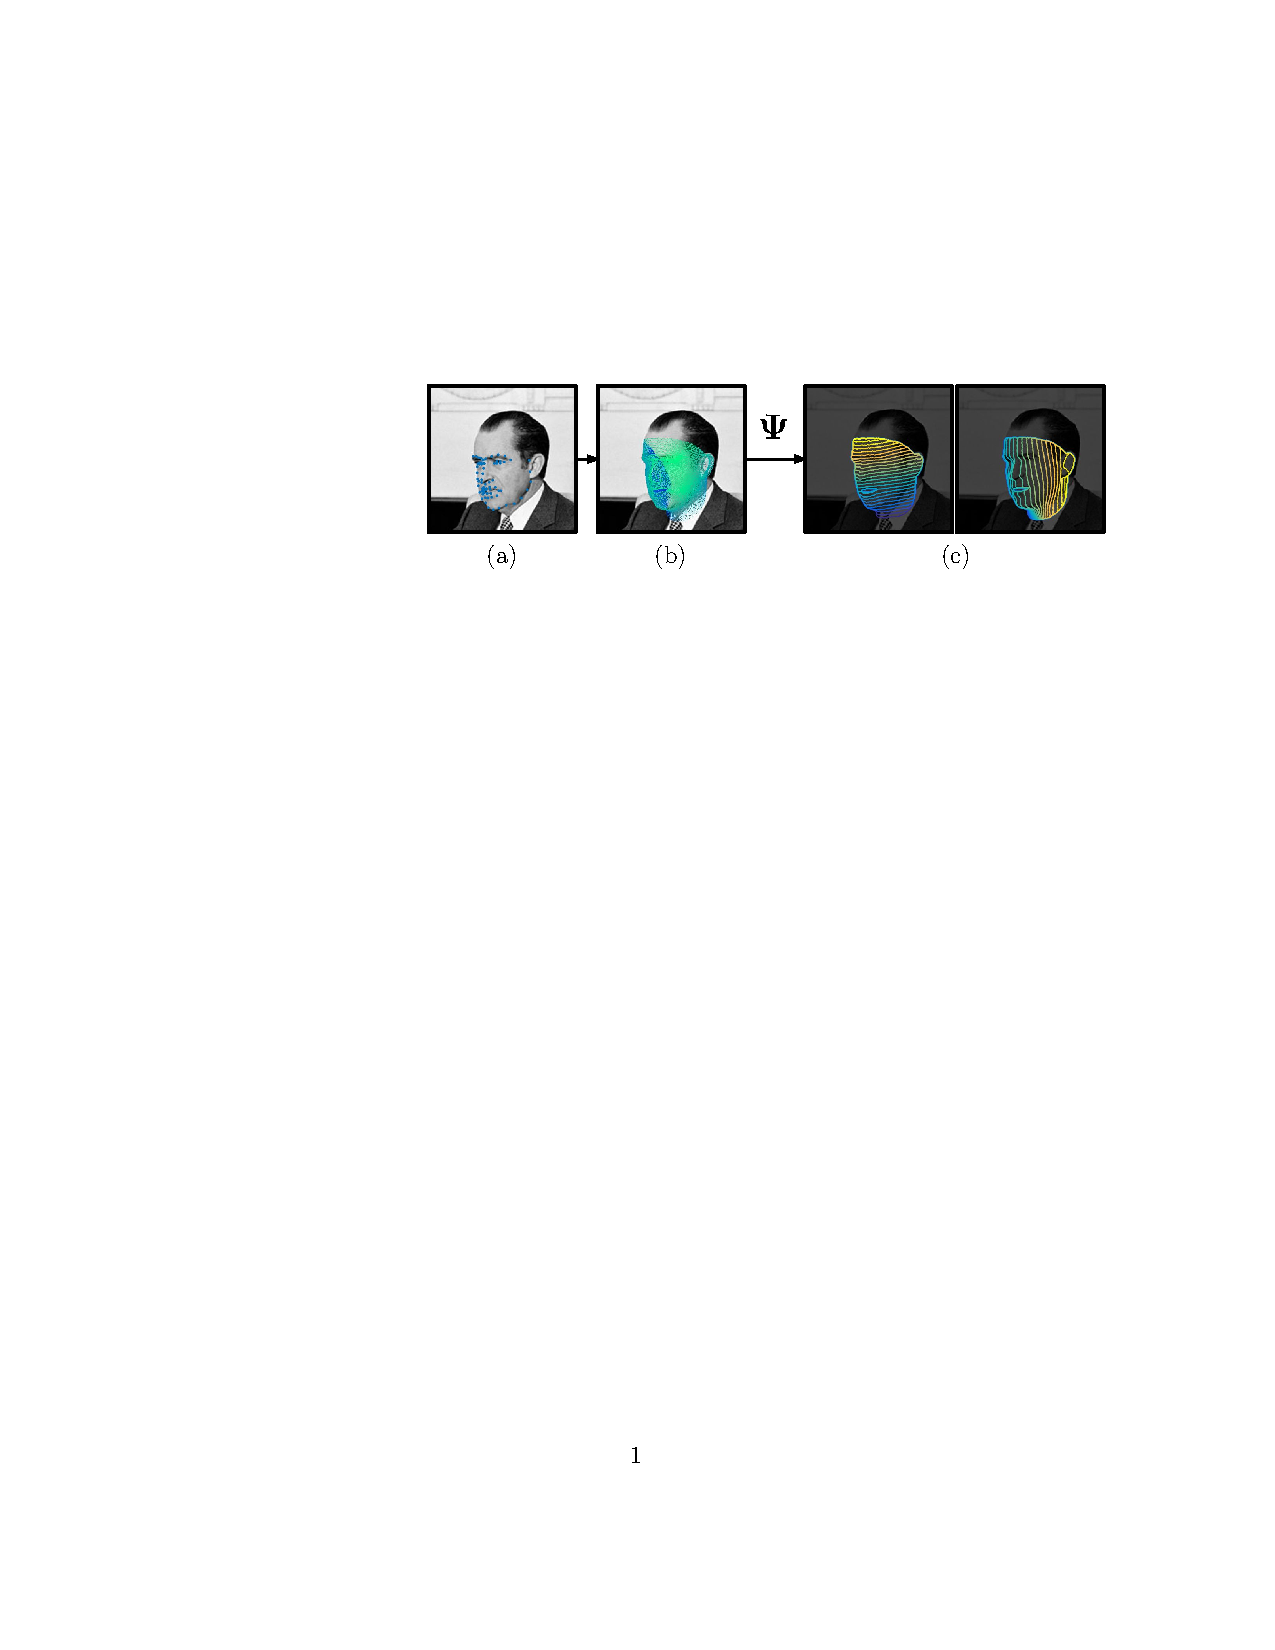
\includegraphics[trim={7.2cm 18.3cm 2.7cm 6.5cm}, clip, width=\linewidth]{Figures/Obtaining_GT}
\caption{Ground-truth generation: \emph{(a)} Annotated landmarks. \emph{(b)} Template shape morphed based on the landmarks. \emph{(c)} Deformation-free coordinates (${u^h}$ and ${u^v}$), obtained by unwrapping the template shape, transferred to image domain. }

\label{fig:GT}
\end{figure}

The mapping $\psi$ is obtained via the cylindrical unwrapping described in \citep{booth2014optimal}. Thanks to the cylindrical unwrapping, we can interpret these coordinates as being the horizontal and vertical coordinates while moving on the face surface: ${u}_j^h \in [0,1]$ and ${u}_j^v \in [0,1]$. Note that this semantically meaningful parameterization has no effect on the operation of our method.
As  illustrated in \ref{fig:GT}, once the transformation from the template face vertices to the morphed vertices is established, the  $\bm{u}_j$ coordinates of each visible vertex on the canonical face can be transferred to the image space. This establishes the ground truth signal for our subsequent regression task.

\subsection{Supervision for the human body template}

We use the recently proposed "Unite the People" (UP) dataset~\citep{lassner2017unite}, which provides a 3D deformable human shape model \citep{loper2015smpl} in correspondence with images from LSP \citep{Johnson10}, MPII~\citep{andriluka14cvpr}, and FashionPose~\citep{dantone2013human} datasets. The dataset is obtained by solving an optimization problem of~\citep{bogo2016keep} to fit the surface given annotated landmarks and manually obtained segmentation masks for human bodies. The fits are filtered through crowdsourcing by manual elimination bad samples resulting into a total of 8515 images.
%
In order to handle the complex geometry of the human shape, we manually partition the surface into 25 patches each of which is isomorphic to the plane. Each vertex on the mesh is assigned a patch label, $I$. We establish a deformation-free coordinate system for each patch by applying multidimensional-scaling to corresponding vertices. This is followed by a normalization to obtain fields $U,V \in [0,1]$.  The $I$ ,$U$ and $V$ fields on the SMPL model\citep{loper2015smpl} is presented in Fig.~\ref{fig:IUV}.
%

%
 

\begin{figure}[h!]
\begin{center}
   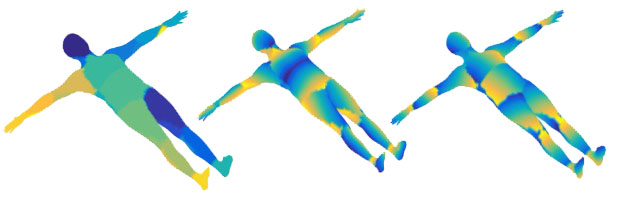
\includegraphics[width=1 \linewidth ]{Figures/IUV_Figure3}
\end{center}
   \caption{ \textit{Top:} Index, U and V fields displayed on the SMPL model. \textit{Bottom:} Dense correspondence results presented as input image fused with estimated UV coordinates, estimated UV coordinates and groundtruth UV coordinates respectively. A customized colour-coding is used for a clear demonstration of correspondence.}
\label{fig:IUV}
\end{figure}

 

%%%%%%%%%%%%%%%%%%%%%%%%%%%%%%%%%%%%%%%%%%%%%%%%%%%%%%%%%%%%%%%%%%%%%%%%%%%%%%%%%%%%%%%%%%%%%%%%%%%%%%%%%%%%%%%%%%%%%%%%%%%%%%%%%%%%%%%%%
